\section{Task-based evaluation}
\label{sec:task-eval}

\definecolor{key0}{RGB}{242,240,247}
\definecolor{key1}{RGB}{203,201,226}
\definecolor{key2}{RGB}{158,154,200}
\definecolor{key3}{RGB}{106,81,163}
\newcommand\crule[1]{\textcolor{#1}{\rule{7pt}{7pt}}}

\begin{table*}[t]
  \centering
  \caption{
    This table shows the summary of the task-based evaluation. I extended the discrete 
    data-focused tasks of Amar, Eagan, and Stasko~\cite{Amar:2005} to directly address
    continuous data, with the exception of ``sort'' (see \autoref{sec:task-eval}). 
    The table shows the scores from our qualitative results inspection as well as
    the expert study on a scale from
    ``none''~\crule{key0}, ``partially''~\crule{key1}, ``mostly''~\crule{key2},
    to ``fully''~\crule{key3}
    where
    ``none'' means that the task is not addressed at all and ``fully'' means 
    that this
    task is directly supported by this view. There are quotes of
    the general description from Amar, Eagan, and Stasko's paper in the ``discrete''
    column for reference. 
  }
  \label{tbl:task_list}
  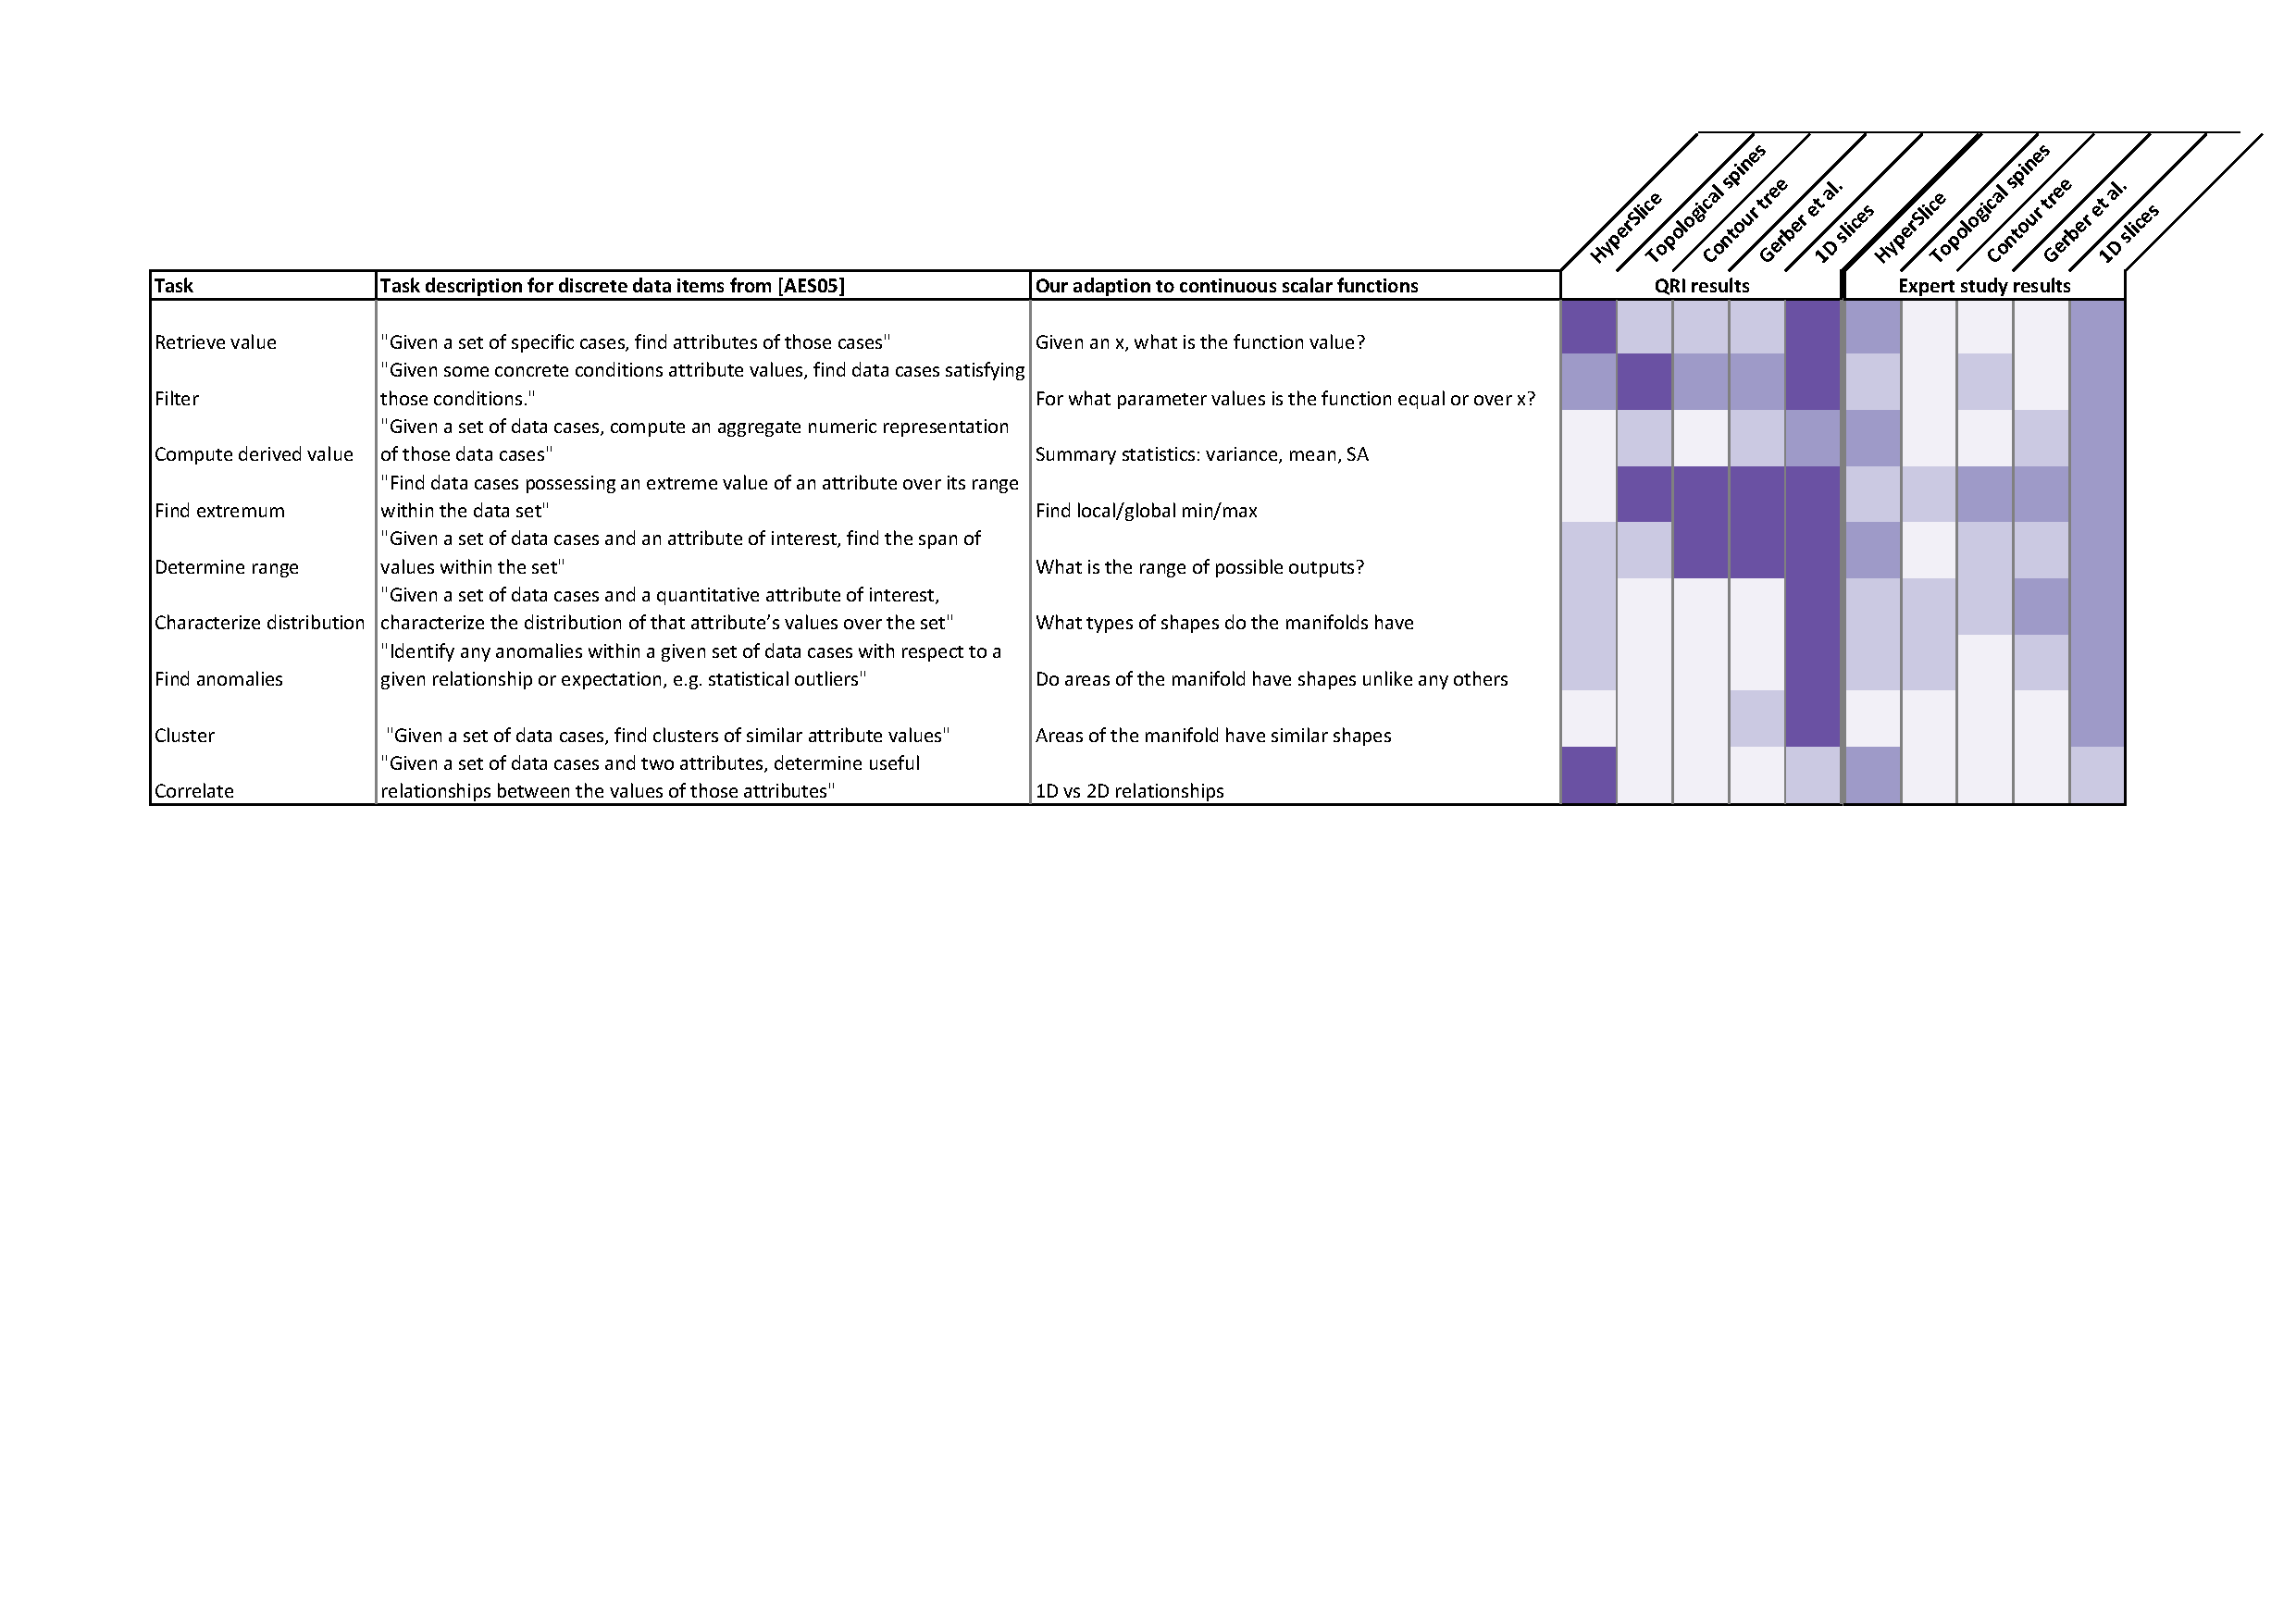
\includegraphics[width=\textwidth]{sp_task_list.pdf}
\end{table*}

\begin{figure}[tb]
  \centering
  \subcaptionbox{HyperSlice~\cite{Wijk:1993}\label{fig:compare:hs}}
    [0.48\textwidth]
    {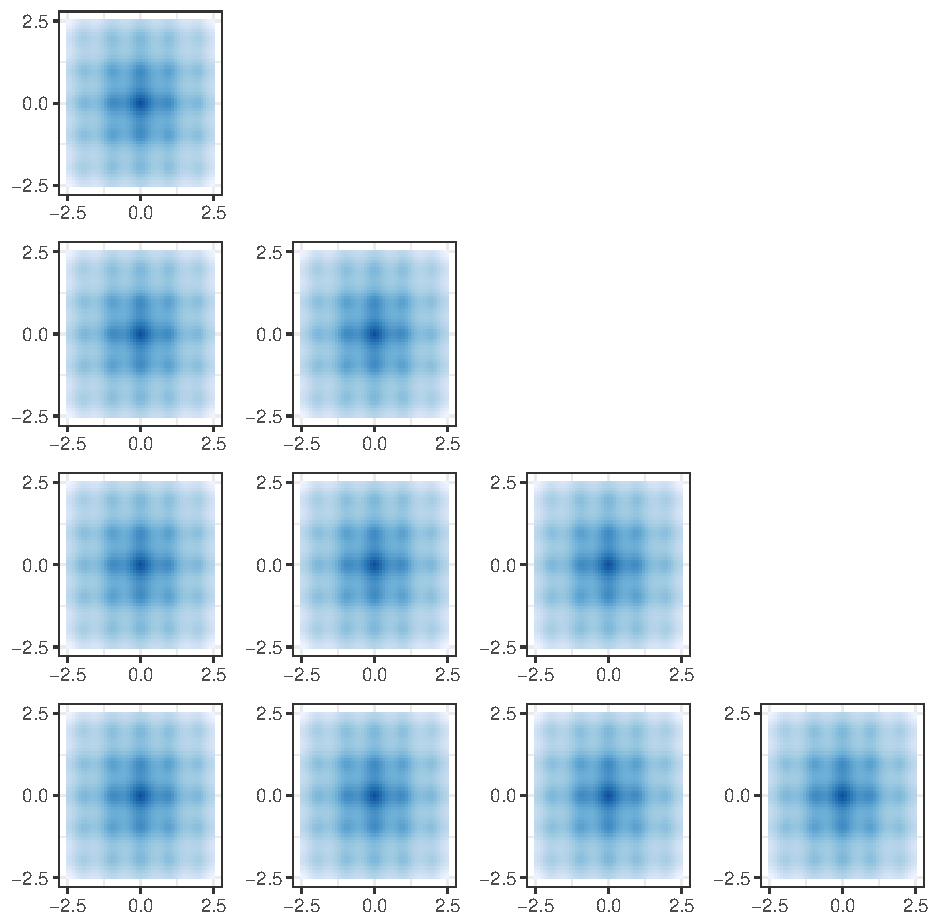
\includegraphics[width=0.17\textwidth]{ackley_5d_hs.pdf}}
  \hfill
  \subcaptionbox{Topological spine~\cite{Correa:2011}\label{fig:compare:ts}}
    [0.48\textwidth]
    {
\includegraphics[width=0.17\textwidth]{topo_spine.pdf}}
  \\
  \subcaptionbox{Contour tree~\cite{Carr:2003}\label{fig:compare:ct}}
    [0.48\textwidth]
    {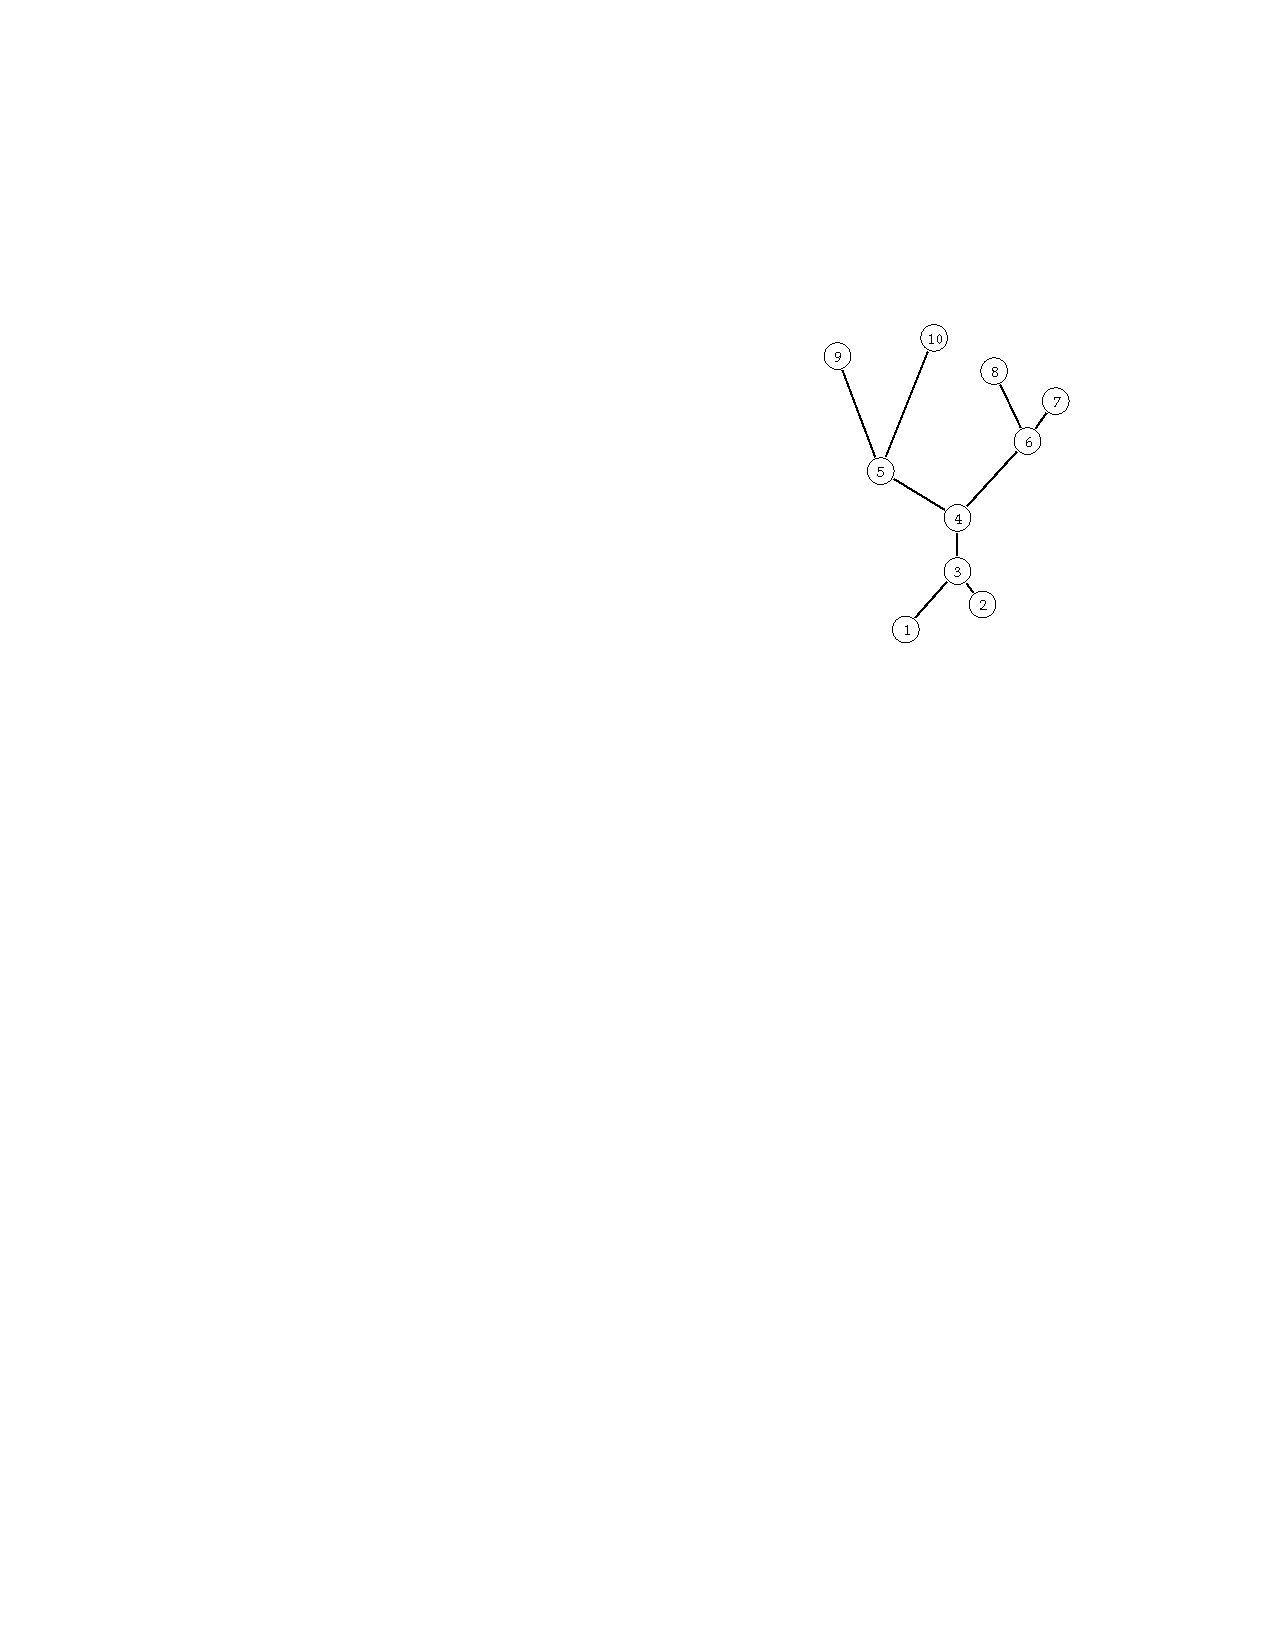
\includegraphics[width=0.17\textwidth]{contour_tree.pdf}}
  \hfill
  \subcaptionbox{Gerber et al.~\cite{Gerber:2010}\label{fig:compare:gerber}}
    [0.48\textwidth]
    {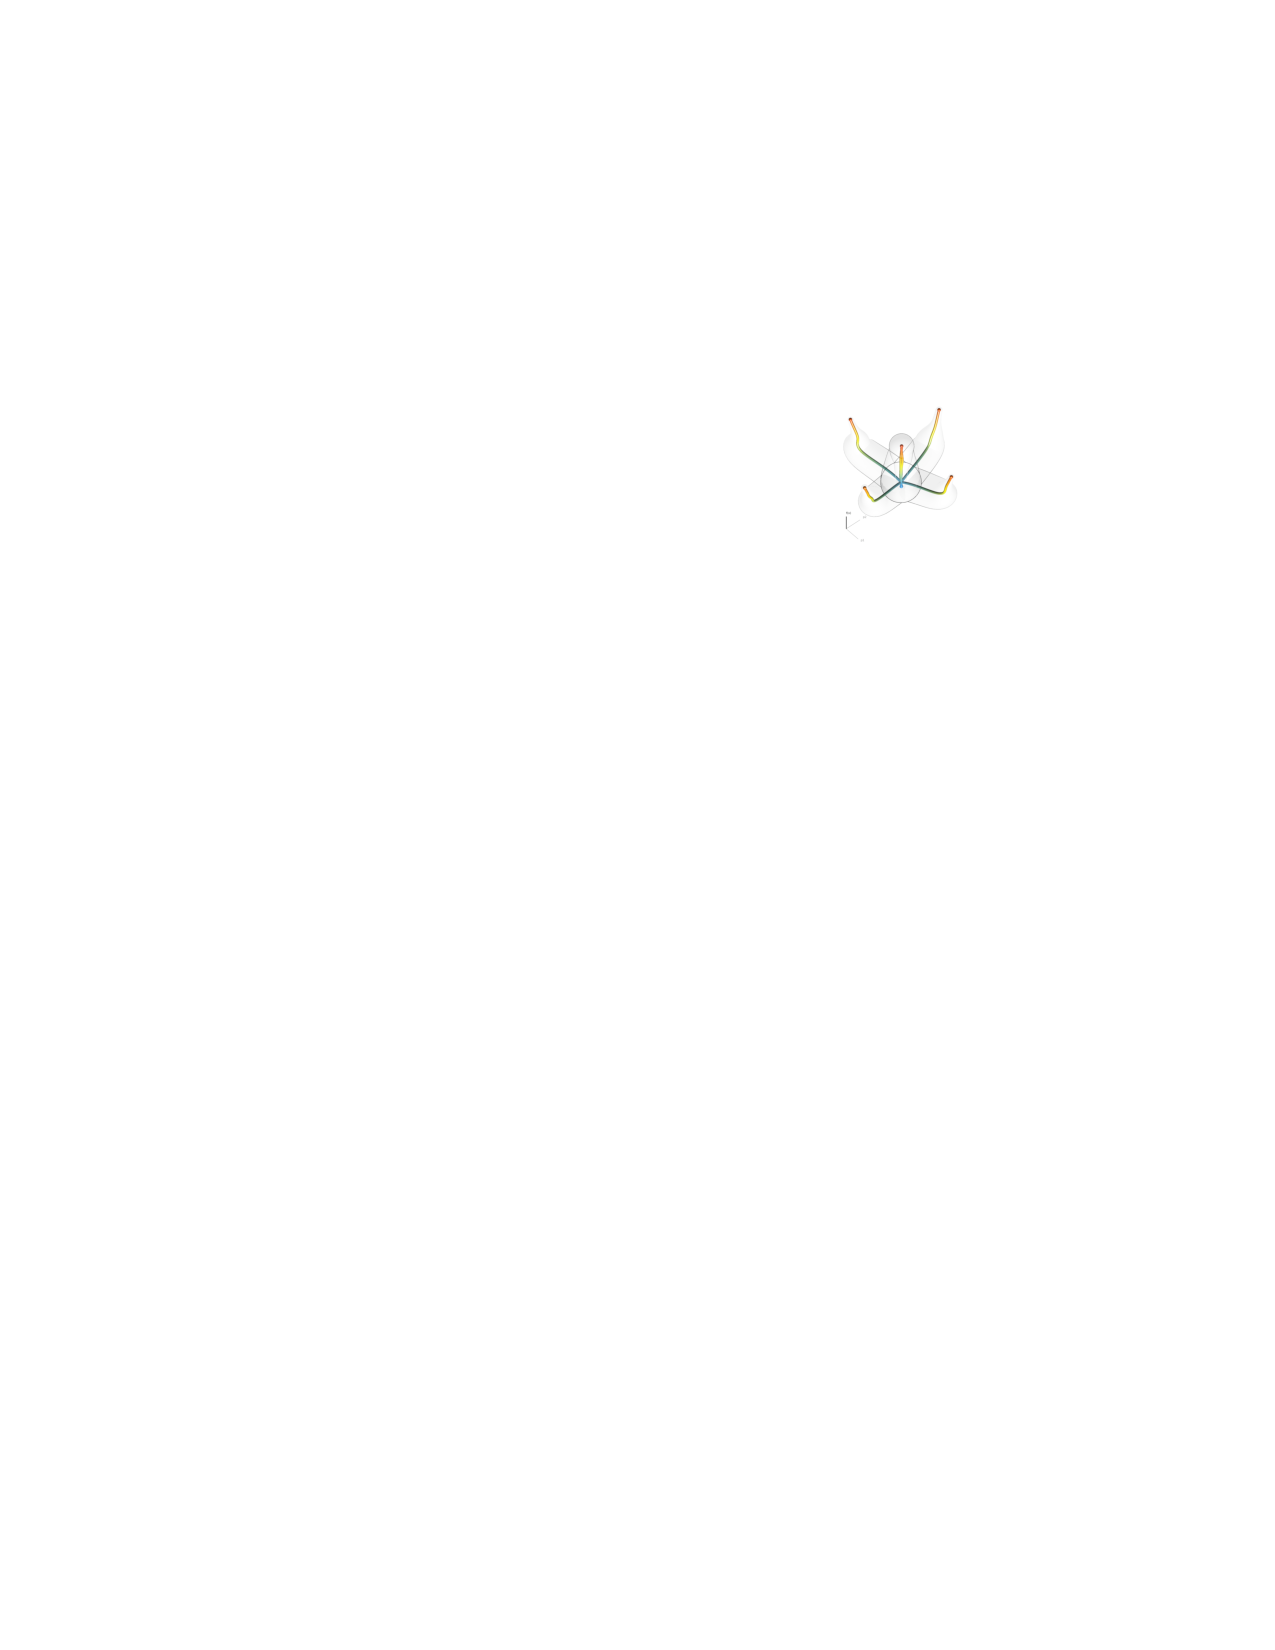
\includegraphics[width=0.17\textwidth]{gerber_ms.pdf}}
  %~
  %\subcaptionbox{1D slices\label{fig:compare:slices}}
    %[0.15\textwidth]
    %{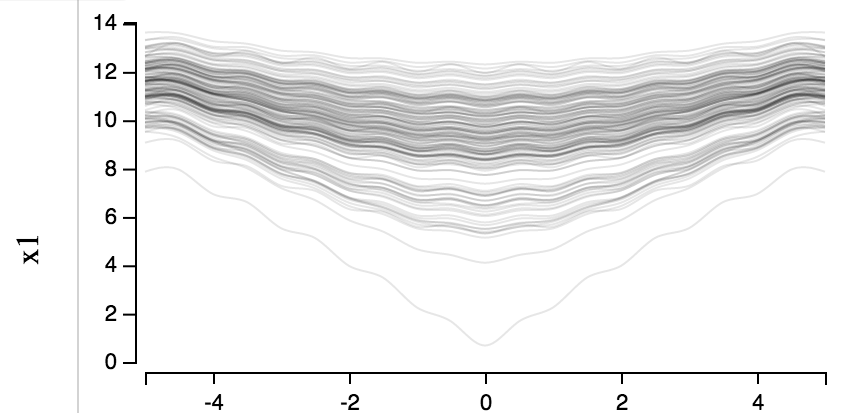
\includegraphics[width=0.1\textwidth]{images/4d_ackley_150slices.png}}
  \caption{
    The four techniques we used to compare with 1D slices. With
    the exception of HyperSlice, the images are from the respective papers and show different datasets used in their context.
  }
  \label{fig:compare}
\end{figure}

I first evaluate 1D slices in terms of their flexibility to deal with a broad
set of different low-level tasks.  Task taxonomies give a basis for comparing
visualization techniques to each other~\cite{Munzner:2014}.
If a technique addresses a large number of tasks, that is usually a good
indicator of its flexibility.  Over the last years, many different taxonomies
have been proposed~\cite{Amar:2005,Brehmer:2013,Heer:2012,Sedlmair:2014}.
However, to the best of my knowledge, none of these taxonomies thus far had a
dedicated focus on the visual analysis of multi-dimensional \textit{continuous}
data. I thus took a popular taxonomy for tasks on discrete data, by Amar,
Eagan, and Stasko~\cite{Amar:2005}, and extended each of their task categories
to directly address continuous data. This is an initial step towards
more consideration of multi-dimensional continuous data as a first class
citizen when developing task hierarchies.

Using this list of tasks, I compare 1D slices to other state of the art
techniques for multi-dimensional continuous data: HyperSlice~\cite{Wijk:1993},
topological spines~\cite{Correa:2011}, contour trees~\cite{Carr:2003}, and the
technique by Gerber et al.~\cite{Gerber:2010} (see \autoref{fig:compare}).  We
refer to topological spines, contour trees, and the work by Gerber et al.\ as
topological techniques when it makes sense to compare them as a group.
We evaluate based on all tasks, except for ``sort'', for which I could not
find a suitable extension to continuous functions.  The guiding theme in the
extensions is that users want to view the relationship of independent variables
to the dependent variable and to see how the dependent variable changes with
respect to the independent values.  The extensions are shown in
\autoref{tbl:task_list} along with the results of two investigations we
conducted based on them, as detailed in the following section.
\subsection{Study design}

To perform a task-based evaluation, I investigated the different techniques in two different ways.
First, I used a \textit{qualitative result inspection}
approach~\cite{Isenberg:2013}. 
I iteratively analyzed the techniques with different datasets and summarized
our discussion and analysis on a four point scale:
``None'' means that it is not possible to perform the task with the technique,
``partly'' means that it requires major interaction with the view to accomplish
the task, ``mostly'' means that one can accomplish the task with little
interaction, and ``fully'' means that this task is directly addressed by the
technique. 

Second, in order to get a more objective judgment I also asked 
\textit{four visualization experts} familiar with examining multi-dimensional spaces like
parameter space exploration to examine the eight datasets with different
techniques and rate how well each task can be accomplished with each technique
on the same scale. \autoref{fig:compare} shows the averaged results along with the
results of the qualitative result inspection in \autoref{fig:compare}.

For the techniques, I use my own implementation of HyperSlice and topological
spines since no code was available. I used the \texttt{msr} R
package~\cite{Gerber:2012} which implements the algorithm of Gerber et
al.~\cite{Gerber:2010}. For the contour tree I used the \texttt{libtourtre}
library and then rendered the trees using GraphViz using the
Sugiyama~\cite{Gansner:1993} layout.  As datasets, I chose the 2D sinc
function, 5D Rosenbrock~\cite{Rosenbrock:1960} function, 6D Ackley function, a
26 node hidden layer neural network built on the Boston housing
dataset~\cite{Lichman:2013}, a support vector machine with Gaussian kernel
built on the housing dataset, the fuel 3D volume dataset~\cite{Roettger:2017},
and the neghip 3D volume dataset~\cite{Roettger:2017}.  
Not all datasets could be rendered with all techniques due to software errors.

\subsection{Results}\label{sec:task-solutions}

In this section, I summarize our discussion about the strengths and weaknesses
of each technique in terms of performing the task.  For more details, there is
also a website that contains details of how each visualization technique can
solve each task. The website is available at
\url{http://sliceplorer.cs.univie.ac.at}.

%\msnote{TO-DISCUSS why is extending tasks from discrete to continuous domain a valid approach?}

\textbf{Retrieve value}:\label{retrieve-value}
In the discrete case, the user should be able to look at a point and get the
detailed values of it. In the continuous case we are interested in what the
function value is for a certain input parameter setting. All the techniques
support this although with the topological methods this is only possible for
the extrema and saddle points as all other points are filtered out. For
example, there could be many points between node $4$ and $5$ in the contour
tree (\autoref{fig:compare:ct}). With
slicing techniques, both 1D and 2D, the values can be read directly off the
chart. Of course, for all techniques the adding of interaction, such as a tooltip, can make retrieving concrete values even easier. 

\textbf{Filter}:\label{filter}
Amar, Eagan, and Stasko describe this task as a general filtering query on data points.
In the continuous case, the user wants to understand the outputs of the
function. This is a query as to where the function value is in a certain range.
With continuous data this is the domain of isosurface extraction.
This is possible with slicing techniques by visual examination.
With HyperSlice, though, one must be careful to view sufficient focus points to
get a general idea of where the function equals certain values.  Topological
spines also shows this directly and they use concentric areas 
(\autoref{fig:compare:ts}) to give a
general idea of the area that a particular value range takes up. The other
topological techniques allow one to see if a certain value is possible, for
example, we can see that the function represented by the contour tree in 
\autoref{fig:compare:ct} takes the values greater than 4 somewhere by seeing 
that there are edges from node 4 to nodes 5 and 6. However,
there is no relation back to the parameter settings that will produce these
values. 

\textbf{Compute derived value}:\label{compute-derived-value}
The direct interpretation of this task to continuous data is to compute derived
value results about the curves 
%\msnote{TO-DISCUSS: the curves? all 1D ones for one dimension? What about derived values that summarize the entire function?} 
like mean and variance. Many of these values can
also be perceived visually.  Topological methods compute the persistence value
between the function to determine what to show but with the exception of
topological spines this is hidden from the user. Topoplogical spines show a
graph of the persistence and ``saturated persistence'' which allows the user
to select which nodes to filter.
Projections of 1D curves allows us to see the distribution.
In
\autoref{fig:walkthrough}c we can see that there are very few function values
around the global minimum and the function has two types of behavior: a
periodic sine wave across the domain and a general parabola shape.

\textbf{Find extremum}:\label{find-extremum}
All the topological techniques we evaluated support this in some
way. With HyperSlice one needs substantial guidance on setting the focus point to find
extrema (like a histogram of function outputs). % or a gradient widget.  Since
1D slices is a global technique showing all slices at once, one can find
extrema by inspecting the graphs.
% see this
%directly since the slices are projected. Extreme values can be seen visually.
As previously mentioned, topological methods are purpose built to extract
extrema from continuous data. For example, it is easy to see that the function
using the method by Gerber et al.\ (\autoref{fig:compare:gerber}) has five
maxima and the function of the contour tree (\autoref{fig:compare:ct}) has four
maxima.

\textbf{Determine range}:\label{determine-range}
Amar, Eagan, and Stasko describe this as finding the range of possible values
for a particular attribute. There is really only one attribute of interest: the
values of the multi-dimensional scalar function. Any view from which we can
read the global minimum or the global maximum allows us to do this. Contour
trees, Gerber et al., and 1D slices all allow us to read these off the view.
Topological spines either show the global maximum \emph{or} the global minimum,
but not both.  HyperSlice has no way to do this directly by adjusting the focus
point.  However, one expert noticed that they could simply read the range of
the function off of the color legend.

\textbf{Characterize Distribution}:
\label{characterize-distribution}
Here again there is one key value of interest that we want to characterize: the
function value.  This requires a global view.  Projections of slices directly
show how the function slices are distributed.  We can see in
\autoref{fig:walkthrough}d that there are very few function values around the
global minimum but many around high values. It would be difficult to use
HyperSlice to truly understand the distribution of values. The user would
somehow have to browse around the focus points and then memorize the function
values. Topology throws away the spatial element and just shows the
relationships between extrema and saddles.

\textbf{Find anomalies}:\label{find-anomalies}
%\msnote{TO-DISCUSS what does an outlier mean in continuous lands? Is it really about shapes? Or is it about spiky-ish behavior?}
Anomalies in the discrete case are single point outliers. While that is also
possible in the continuous case, we may also have entire parts of the function
that are unlike any other part. These should also be identified.
In a global view like projected 1D slices these will show up visually. The
slices will stand out from the rest similar to other projection-based
techniques like scatterplots. With HyperSlice we must browse around until we
can see one directly. However, we will see it if we can find it. Topological
methods will only show extrema in terms of maxima or minima values but not
shape and hence mask anomalies and outliers.

\textbf{Cluster}:\label{cluster}
Since we are looking at manifold behaviors, we want to be able to group the
functions into areas of similar behavior. For example, are they monotonically
increasing or decreasing? Furthermore, can we find areas where the variance
changes? The topological technique of Gerber et al.~\cite{Gerber:2010} was
created to address just this. They split the function
into areas of monotonic behavior and then show a line indicating how those
monotonic regions are related to each other. However, the way they
reconstruct the function between extrema and saddle points does not allow us to
view the variance between these points as the 1D slice view
allows. Clustering the 1D slices tries to split the slices into groups of
similar behavior (see \autoref{fig:cluster:clustered}).

%\begin{figure}
  %\centering
  %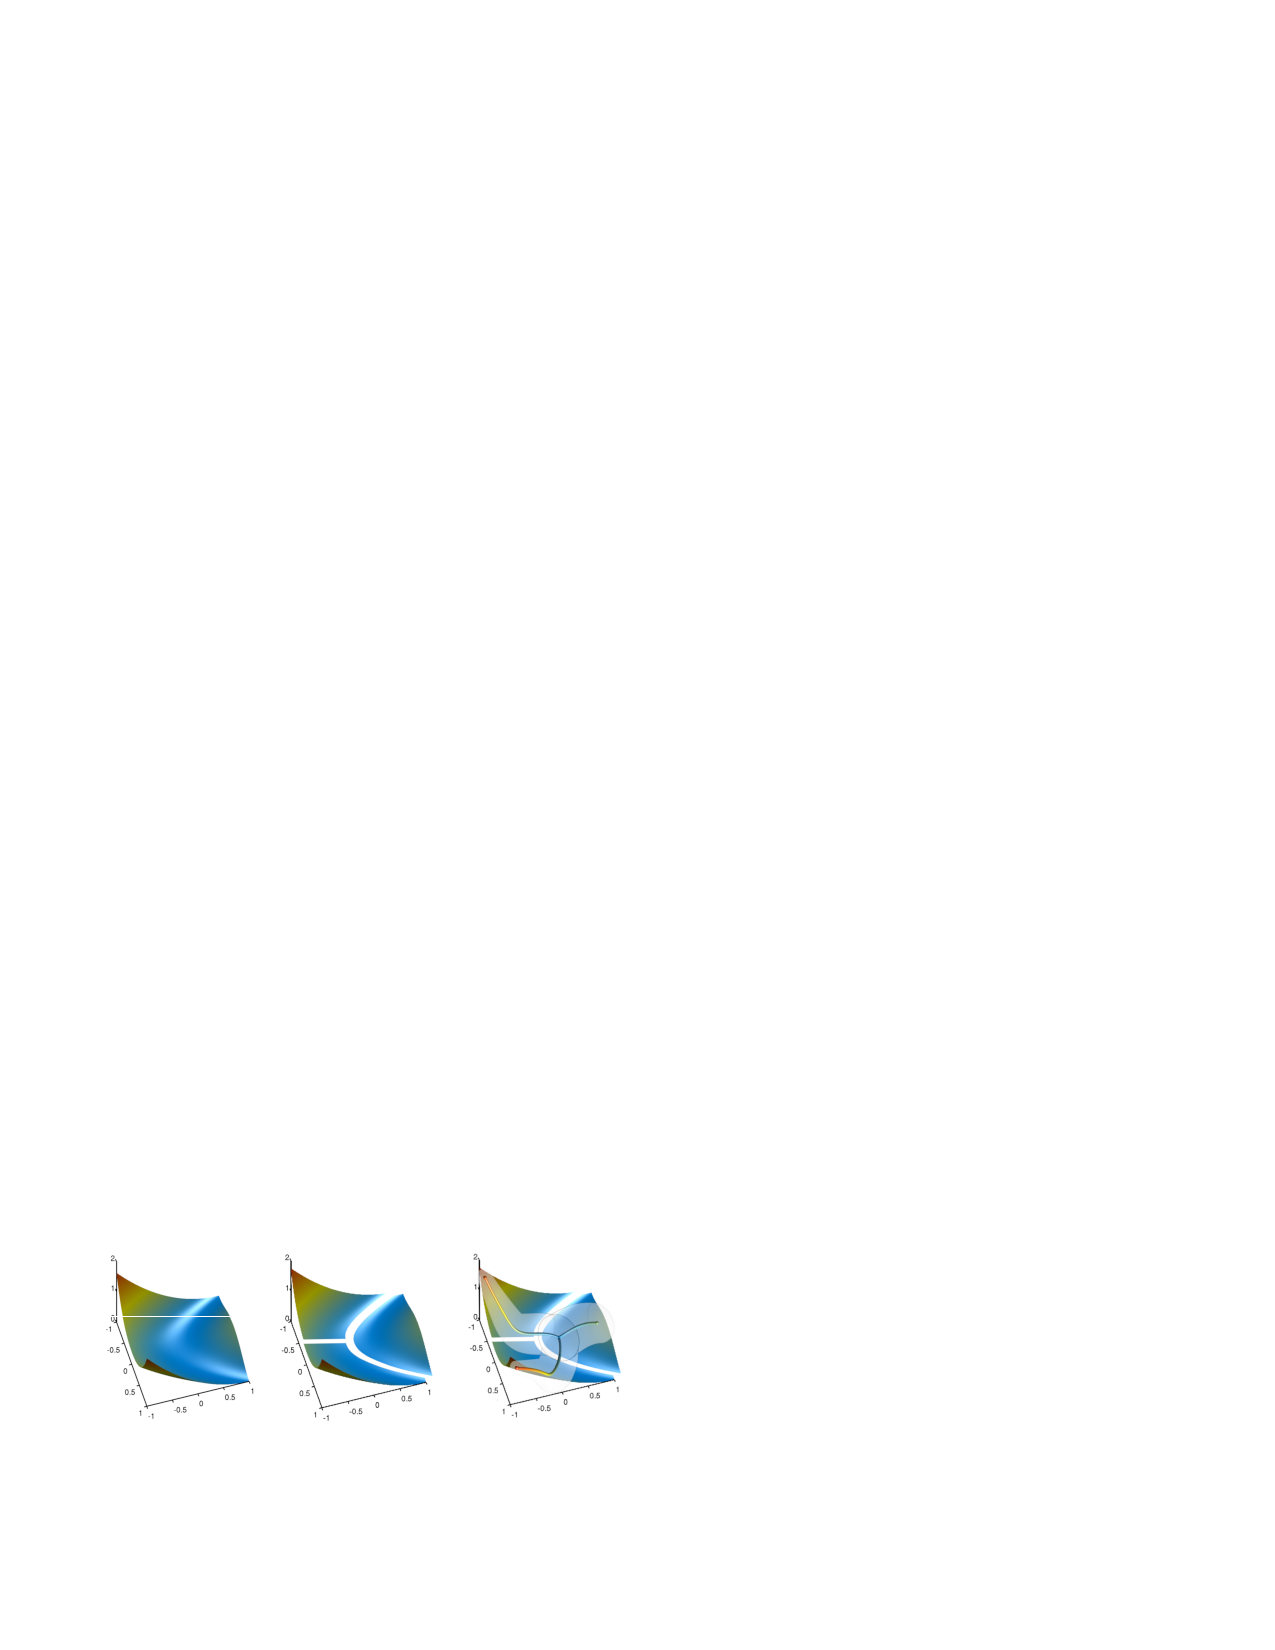
\includegraphics[width=\columnwidth]{images/gerber_evolution.pdf}
  %\caption{
    %How the method of Gerber et al.\ visualizes a function. They take a 
    %function (left image), decompose it into areas of monotonic behavior 
    %(center image), approximate each region with a regression model (right
    %image), and then show this regression model to the user.
    %(image from \cite{Gerber:2010}).
  %}
  %\label{fig:gerber}
%\end{figure}

\textbf{Correlate}:\label{correlate}
Finally, we consider correlation. In the discrete data case the goal is to find
correlation between attributes. With continuous data, we already have a
dependency between the independent and dependent variables. What we would like
to learn is how many variables have an influence on the function. With 2D views
(that only HyperSlice provides) one can see both 1D and 2D interactions with
the function. We can see that the function in \autoref{fig:compare:hs} has
radial behavior so the function value depends on both 1D and 2D interactions.
None of the other techniques are capable of showing 2D interactions between
parameters.

\subsection{Summary}

From the summary in \autoref{tbl:task_list} we can see that the 1D slices
technique addresses more of the tasks than any other technique.  It is not
always the highest performing view though.  HyperSlice is the only technique 
evaluated that could show more than one-dimensional interactions but it does
not do well on global tasks like extrema detection. The various topological
techniques directly address tasks related to extrema detection and comparison
but do not perform as well on others. 
%\ttwnote{should the following go in limitations?}
The experts often commented that they felt they needed more knowledge about
what exactly the topological techniques were doing in order to interpret
the results. Thus, the ratings for these techniques may be artificially low.
%\ttwnote{However, given the difficulty that experts had with the technique,
%this does not bode well for the general public.}
I conclude that 1D slices are a
very flexible technique indeed.  

